\documentclass[14pt,dvipdfmx]{beamer}

% Beamerの設定
\usetheme{Boadilla}
% Beamerフォント設定
\usepackage{txfonts} % TXフォント
% \usepackage[deluxe,uplatex]{otf} % 日本語多ウェイト化
\usepackage[deluxe]{otf} % platexの場合はこちら
\usepackage{pxjahyper} % PDF目次文字化け回避(platexでは不要)
\renewcommand{\familydefault}{\sfdefault}  % 英文をサンセリフ体に
\renewcommand{\kanjifamilydefault}{\gtdefault}  % 日本語をゴシック体に
\usefonttheme{structurebold} % タイトル部を太字
\setbeamerfont{alerted text}{series=\bfseries} % Alertを太字
\setbeamerfont{section in toc}{series=\mdseries} % 目次は太字にしない
\setbeamerfont{frametitle}{size=\Large} % フレームタイトル文字サイズ
\setbeamerfont{title}{size=\LARGE} % タイトル文字サイズ
\setbeamerfont{date}{size=\small}  % 日付文字サイズ


% フラットデザイン化
\setbeamertemplate{blocks}[rounded] % Blockの影を消す
\useinnertheme{circles} % 箇条書きをシンプルに
\setbeamertemplate{navigation symbols}{} % ナビゲーションシンボルを消す
\setbeamertemplate{footline}[frame number] % フッターはスライド番号のみ

% タイトルページ
\setbeamertemplate{title page}{%
  \vspace{2.5em}
  {\usebeamerfont{title} \usebeamercolor[fg]{title} \inserttitle \par}
  {\usebeamerfont{subtitle}\usebeamercolor[fg]{subtitle}\insertsubtitle \par}
  \vspace{1.5em}
  \begin{flushright}
    \usebeamerfont{author}\insertauthor\par
    \usebeamerfont{institute}\insertinstitute \par
    \vspace{3em}
    \usebeamerfont{date}\insertdate\par
    \usebeamercolor[fg]{titlegraphic}\inserttitlegraphic
  \end{flushright}
}

% graphicx.sty
\usepackage{graphicx}

% Algorithm系
\usepackage{algorithm}
\usepackage[noend]{algorithmic}
\algsetup{linenosize=\color{fg!50}\footnotesize}
\renewcommand\algorithmicdo{:}
\renewcommand\algorithmicthen{:}
\renewcommand\algorithmicrequire{\textbf{Input:}}
\renewcommand\algorithmicensure{\textbf{Output:}}

% Tikz
\usepackage{tikz}
\usetikzlibrary{positioning,shapes,arrows}

% 定理
\theoremstyle{definition}
\newtheorem{thm}{Theorem}
\newtheorem{lem}{Lemma}
\newenvironment{mythm}{\begin{alertblock}{定理}}{\end{alertblock}} %自分の結果は赤色で表示

\AtBeginSection[]{
  \frame{\tableofcontents[currentsection, hideallsubsections]} %目次スライド
}

%% =====================================================================
\title{全体ゼミ}
\author{大石純平(筑波大学)}
\date{2015/4/24}
\institute{プログラム論理研究室}

\begin{document}
\maketitle

\begin{frame}{Offshoreとは}
  \center
  \Huge{委託}
\end{frame}

\begin{frame}{Offshoreで目指すこと}
  \center
  \large
  \begin{itemize}
  \item <1-> 人間が書きやすい高級な言語から,低級な言語へ変換を行う.
  \item <2-> 変換後のコードが実行効率を犠牲にすることなく,低級な言語が得意な最適化を行うことができれば嬉しい.
  \item <3> 一つのコード生成器から,目的に応じた様々なコードを生成する.
  \end{itemize}
\end{frame}

\begin{frame}{使用した言語}
  \center
  \large
  \begin{block}{BER MetaOCaml}
    マルチステージプログラミング言語
  \end{block}

  \normalsize
  \begin{itemize}
  \item <2-> コードを生成する前に,生成したコードの安全性を保証.
    \begin{itemize}
    \item <3> 生成したコードは実行時エラーが起きない.
    \end{itemize}
  \end{itemize}
\end{frame}
\begin{frame}{今回用いたシステム}
  \center
  \Huge
  明日奈システム
  \pause
  \center
  \normalsize
  高島さんの作ったやつ
\end{frame}

\begin{frame}{今回用いたシステム}
  \begin{figure}[ht]
    \centering
    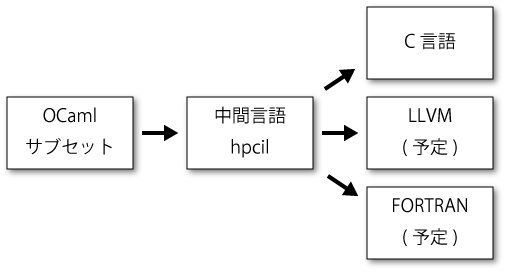
\includegraphics[width=100mm]{./img/figure1.png}
  \end{figure}
\end{frame}

\begin{frame}{実験の趣旨}
  最適化を行わない場合のOCamlのコードと
  変換後のC言語のコードとの実行時間を調べたい.
\end{frame}
\begin{frame}{実験内容}
  gcc -O3, gcc, clang -O3, clang, ocamlc, ocamlopt によってコンパイルしたものをそれぞれ5回実行し,その結果の平均を求めた.
\end{frame}

\begin{frame}{実験}
  \begin{block}{C}
    \begin{itemize}
    \item clang -O3
    \item gcc -O3
    \end{itemize}
  \end{block}

  \begin{block}{OCaml}
    \begin{itemize}
    \item ocamlopt
    \item ocamlc
    \end{itemize}
  \end{block}
\end{frame}

\begin{frame}{スペック}
  \begin{block}{使用した画像}
    \begin{itemize}
    \item 8k画像 ($768 \times 4320$ pixel)
    \end{itemize}
  \end{block}
  \begin{block}{マシンスペック}
    \begin{itemize}
    \item CPU: Intel Core i7-4790K
    \item コア数: 4
    \item スレッド数: 8
    \item ベース動作周波数: 4.0GHz
    \item L1 キャッシュサイズ: 256KB
    \item L2 キャッシュサイズ: 1024KB
    \item L3 キャッシュサイズ: 8192KB
    \item メモリ: DDR3 16GB 1600MHz
    \end{itemize}
  \end{block}
\end{frame}

\begin{frame}{使用した画像}
  \begin{figure}[ht]
    \centering
    
\includegraphics[width=100mm]{./img/planet.jpg}
  \end{figure}

\end{frame}
\begin{frame}{ネガポジ反転した画像}
  \begin{figure}[ht]
    \centering
    
\includegraphics[width=100mm]{./img/planet_nega.jpg}
  \end{figure}
\end{frame}

\begin{frame}[containsverbatim]{使用したコード}
\begin{verbatim}
.<fun w h inp out ->
  for i = 0 to w*h*3 - 1 do
    out.(i) <- 255 - inp.(i)
  done>.
\end{verbatim}
\end{frame}

\begin{frame}[containsverbatim]{変換したコード}
  \small
\begin{verbatim}
void ngps(int w_1, int h_2, int *inp_3, int *out_4)
{
    int i_5;
    for (i_5 = 0; i_5 <= w_1 * h_2 * 3 - 1; i_5++)
        out_4[i_5] = 255 - inp_3[i_5];
}
\end{verbatim}
\end{frame}


\begin{frame}{実験結果}
  \begin{figure}[ht]
    \centering
    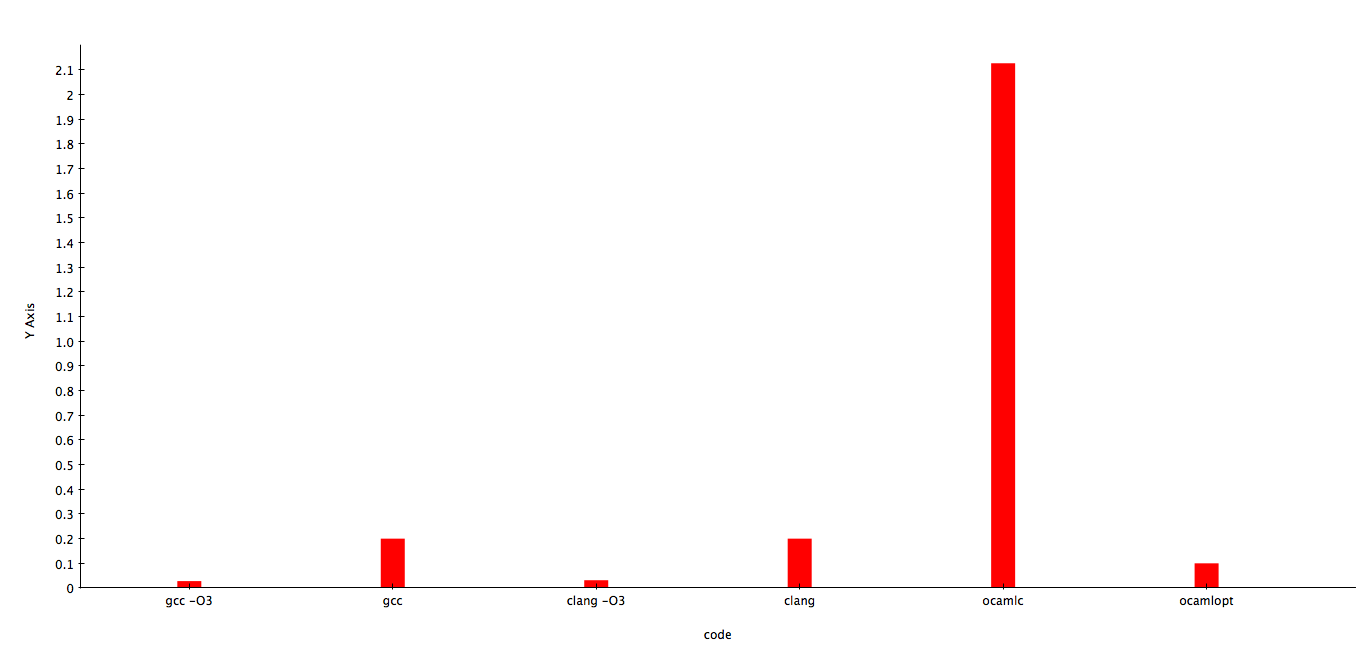
\includegraphics[width=130mm]{./img/time01.png}
  \end{figure}
\end{frame}

\begin{frame}{実験結果}
  \begin{figure}[ht]
    \centering
    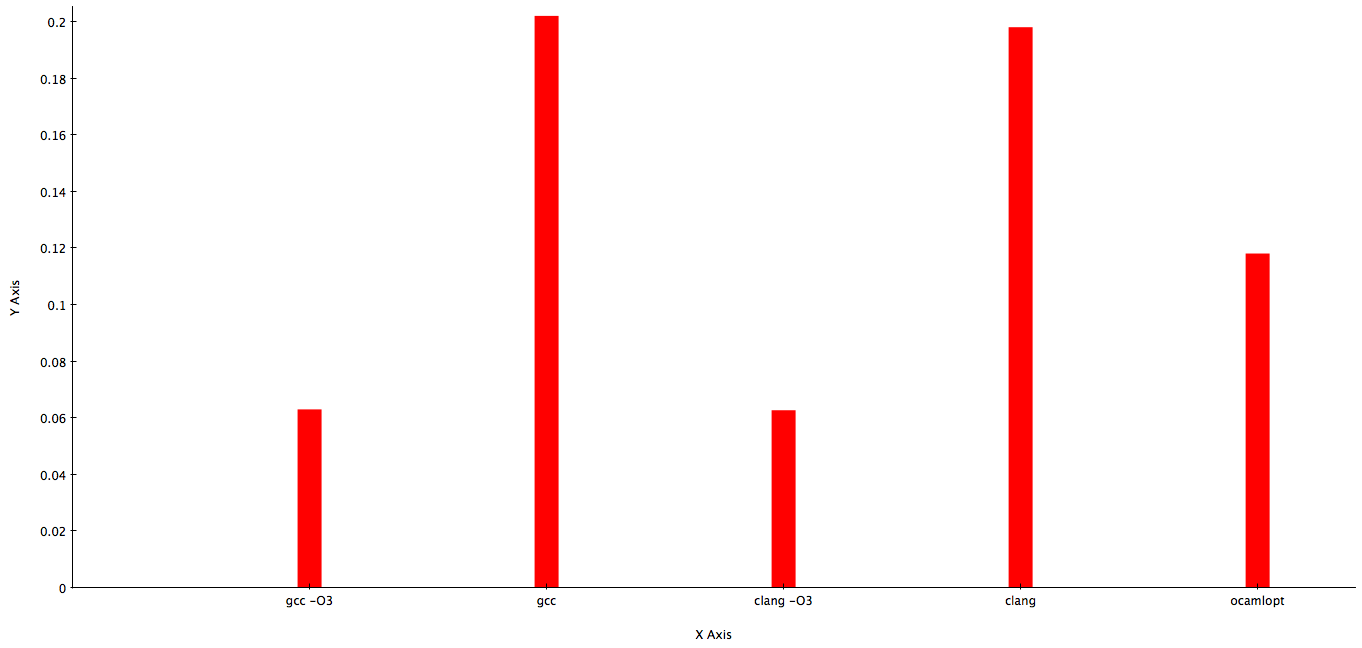
\includegraphics[width=130mm]{./img/time02.png}
  \end{figure}
\end{frame}

\begin{frame}{実験結果}
  \begin{itemize}
  \item gcc -O3 : $0.0629$ [s]
  \item gcc : $0.202$ [s]
  \item clang -O3 : $0.0626$ [s]
  \item clang : $0.198$ [s]
  \item ocamlc : $2.161$ [s]
  \item ocamlopt : $0.118$ [s]
  \end{itemize}
\end{frame}

\begin{frame}{考察}
  \begin{itemize}
  \item ocamlcでのコンパイルによって生成された実行ファイルの実行時間は一番遅い.
  \item ocamloptは健闘しているが,offshoreされたC言語の-O3オプションを付けて生成した実行ファイルの実行時間は,それに比べて2倍ほど速い.
  \end{itemize}

\end{frame}

\begin{frame}{実験結果}

  \begin{table}[htb]
    \scriptsize
    \centering
    \begin{tabular}{|r|c|c|c|c|c|c|c|} \hline
     回数& gcc -O3 [s]&gcc [s]& clang -O3 [s]& clang [s]& ocamlc [s]& ocamlopt [s]\\ \hline
     1& 0.084628 & 0.248957 & 0.083537 & 0.245865 & 2.161121  & 2.161121 \\ \hline
		 2& 0.057468 & 0.190805 & 0.057313 & 0.186081 & 2.160990	& 2.160990 \\ \hline
		 3& 0.057403 & 0.190846 & 0.057324 & 0.185934 & 2.159268	& 2.159268 \\ \hline
		 4& 0.057429 & 0.190796 & 0.057357 & 0.185931 & 2.160954	& 2.160954 \\ \hline
		 5& 0.057414 & 0.190914 & 0.057307 & 0.185922 & 2.159235	& 2.159235 \\ \hline
    \end{tabular}
  \end{table}
\end{frame}

\begin{frame}{考察}
  \begin{itemize}
  \item Cのコンパイラによって生成された実行ファイルは総じて1回目の実行速度が遅い.
  \item 1回目は直接メモリから読み込むから少し遅く,
  \item 2回目以降はキャッシュから読み込むから速いのだろう.
  \end{itemize}
\end{frame}

\begin{frame}[containsverbatim]{実験結果}
  gcc -O3 -S によって出力されたアセンブリコードの一部を示す.
  xmmというものがベクトルレジスターと呼ばれるものである.
\begin{verbatim}
 .L4:
	  movdqu	(%rdx,%rax), %xmm0
	  addl	$1, %esi
	  movdqa	%xmm1, %xmm2
	  psubd	%xmm0, %xmm2
	  movdqu	%xmm2, (%rcx,%rax)
	  addq	$16, %rax
	  cmpl	%esi, %r8d
	  ja	.L4
	  cmpl	%r9d, %edi
	  movl	%r9d, %esi
	  je	.L12
\end{verbatim}
\end{frame}

\begin{frame}{考察}
  \begin{itemize}
  \item gcc -O3 でコンパイルすることにより,SIMD命令が出力された.
  \item clang -O3でも同様にSIMD命令が出力された.
  \item 配列に対して連続アクセスをするようなよくあるパターンだったため,
    gccの自動ベクトル化機構が有効に働いたと考えられる.
  \end{itemize}
\end{frame}

\begin{frame}{前提知識}
  \begin{block}{SIMD命令}
    同じ演算を複数のデータに対して1サイクルで適用する命令
  \end{block}
  \begin{figure}[ht]
    \centering
    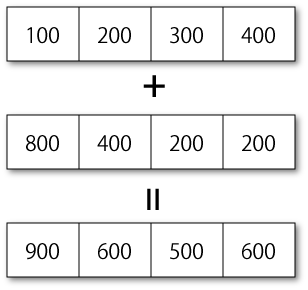
\includegraphics[width=50mm]{./img/figure2.png}
  \end{figure}
\end{frame}

\begin{frame}{前提知識}
  \begin{block}{自動ベクトル化}
    コードをSIMD命令を利用したコードに自動的に変換すること
  \end{block}
\end{frame}



\end{document}